\chapter{Atividades Desenvolvidas e Resultados}\label{chap4}
\thispagestyle{fancy}

Neste capítulo, são descritas em pormenor as atividades realizadas ao longo do período de estágio, as quais se dividiram em duas vertentes principais: a componente de engenharia e desenvolvimento de software (que engloba a modelação de base de dados, desenvolvimento do website e de aplicações empresariais) e a componente prática de hardware (que compreende tarefas manuais de triagem, teste e reciclagem de componentes eletrónicos nas instalações da empresa).

\section{Desenvolvimento de Software e Aplicações}

Esta secção descreve a conceção, arquitetura e implementação das soluções de software que compõem o ecossistema tecnológico desenvolvido para a empresa.

\subsection{Arquitetura Geral do Sistema}

O ecossistema tecnológico foi desenhado sob uma arquitetura distribuída e modular, visando garantir a separação de conceitos, a escalabilidade das aplicações e a facilidade de manutenção a longo prazo. O núcleo da solução assenta num modelo de \textit{Clean Architecture} (ou Arquitetura Cebola) implementado no backoffice, complementado por uma API centralizada que funciona como o único ponto de contacto com a base de dados.

A infraestrutura é constituída por três camadas lógicas principais:
\begin{itemize}
    \item \textbf{Camada de Apresentação (Frontend/Clientes):} constituída pelo Website Institucional em Next.js 15, pela aplicação de Backoffice e pelo Terminal de Pesagem (Kiosk), ambos desenvolvidos em Blazor Server no ecossistema .NET 10.
    \item \textbf{Camada de Serviços (API Central):} uma API RESTful em .NET 10 que expõe os \textit{endpoints} de negócio necessários e assegura que todas as validações, regras e acessos à base de dados ocorrem sob uma mesma lógica corporativa.
    \item \textbf{Camada de Dados e Infraestrutura (Supabase/PostgreSQL):} alojamento na nuvem da base de dados PostgreSQL e do serviço de armazenamento de ficheiros do Supabase.
\end{itemize}

O isolamento das regras de negócio na API central garante que as aplicações clientes (Web, Backoffice e Quiosque) não comuniquem diretamente com a base de dados, reduzindo o risco de acessos não autorizados e facilitando futuras integrações com outros sistemas da empresa.

\subsection{Fluxos Principais da Aplicação}

Para assegurar a digitalização eficiente dos processos da empresa, foram modelados e implementados três fluxos fundamentais:
\begin{enumerate}
    \item \textbf{Fluxo de Submissão e Triagem de Pedidos de Recolha:} O cliente acede à área reservada do website e submete um formulário indicando o material a recolher, anexando fotografias. O pedido entra na base de dados com o estado \textit{Pendente}. O operador, na app de Backoffice, recebe o alerta, analisa os dados e as fotos e agenda a recolha física, alterando o estado para \textit{Agendada}.
    \item \textbf{Fluxo de Pesagem e Integração Física:} No armazém, o motorista descarrega os resíduos. O operador no terminal de pesagem (Kiosk) escolhe a recolha ativa. O operador insere o valor do peso medido no terminal, que submete os dados à API central. A pesagem é associada ao pedido de recolha original, atualizando a conta corrente do cliente.
    \item \textbf{Fluxo de Alteração Cadastral e Auditoria de Segurança:} Visando impedir fraudes e dados cadastrais incorretos na faturação, sempre que o cliente edita os seus dados fiscais ou morada na área reservada do website, a atualização não é imediata. A alteração entra numa tabela de propostas temporárias. O operador de backoffice analisa o pedido e valida. Se aprovar, a API executa a persistência na tabela central de Clientes e cria um registo de auditoria (\textit{audit log}).
\end{enumerate}

\subsection{Modelação da Base de Dados}

A base de dados constitui o núcleo central de toda a infraestrutura tecnológica desenvolvida, sustentando de forma unificada tanto o website institucional (através da área reservada de cliente e do painel de gestão editorial) como as aplicações empresariais de backoffice e do terminal de pesagem. Para responder aos requisitos de consistência, integridade de dados e escalabilidade, optou-se pela utilização de um sistema de gestão de bases de dados relacional, especificamente o PostgreSQL. A base de dados é gerida e alojada na nuvem através da plataforma Supabase, o que confere elevada disponibilidade e simplifica as operações de monitorização e cópias de segurança.

A modelação física e a comunicação com o motor de base de dados foram estruturadas através de uma abordagem \textit{Code-First} suportada pelo Entity Framework Core (EF Core), o mapeador objeto-relacional (ORM) padrão da plataforma .NET. Sob esta metodologia, todo o esquema de tabelas, chaves primárias, chaves estrangeiras e restrições de integridade foi modelado sob a forma de classes de domínio na linguagem C\#. As atualizações estruturais e a sincronização do esquema com o servidor PostgreSQL foram geridas de forma estrita através do sistema de migrações (\textit{migrations}) do EF Core, assegurando a rastreabilidade e a reprodutibilidade do esquema em ambientes de desenvolvimento e produção.

A arquitetura de dados divide-se nas seguintes entidades principais:
\begin{itemize}
    \item \textbf{Cliente:} Armazena os dados de contacto, localização e de identificação necessários para a faturação e conformidade legal das entidades clientes. Esta entidade está associada ao utilizador registado no serviço de autenticação central do Supabase através de um identificador único de utilizador.
    \item \textbf{CodigoLer e Material:} Representam a catalogação regulamentar e comercial de resíduos. A tabela \textit{CodigoLer} armazena os códigos oficiais estabelecidos na Lista Europeia de Resíduos (LER) e a respetiva descrição. A tabela \textit{Material} associa um nome operacional e a informação tarifária aplicável a cada tipo de resíduo sob um código LER.
    \item \textbf{PedidoRecolha:} Regista as solicitações de recolha submetidas pelos clientes através do website ou inseridas manualmente pelos operadores. Guarda o estado de processamento do pedido, notas adicionais, informações de contacto e dados geográficos da recolha. Associa-se aos materiais pretendidos através da tabela de junção \textit{PedidoMaterialPretendido}.
    \item \textbf{Recolha:} Modela o evento logístico de recolha de resíduos. Contém a data programada, o estado de execução, dados geográficos e de contacto para a operação. Relaciona-se com os materiais selecionados para a recolha através da tabela de junção \textit{RecolhaMaterialPreSelecionado}.
    \item \textbf{Pesagem:} Regista as pesagens efetuadas na balança física. Guarda a quantidade líquida pesada, o valor calculado da transação, o material correspondente, o operador que validou a pesagem e a recolha associada.
    \item \textbf{Utilizador e Cargo:} Representam os utilizadores internos do sistema (como operadores de balança, funcionários de armazém e administradores). Cada conta está associada a um cargo, cujas permissões de acesso a funcionalidades do sistema são configuradas de forma granular através de um campo estruturado em formato JSON.
    \item \textbf{KioskDevice e KioskPairingCode:} Suportam a segurança dos quiosques físicos de pesagem. Registam os identificadores exclusivos dos terminais autorizados e gerem os códigos temporários utilizados para emparelhar em segurança novos dispositivos quiosque à infraestrutura central.
    \item \textbf{Noticias e RevisoeseNoticias:} Suportam o sistema de publicação de conteúdos do website institucional, gerindo dados textuais, categorias, referências a imagens de capa e campos destinados à otimização em motores de busca (SEO). A tabela \textit{RevisoeseNoticias} mantém o histórico de modificações para auditoria e reversão.
    \item \textbf{ChatMessage:} Implementa o suporte direto e bidirecional de mensagens entre os clientes e os operadores de backoffice, possuindo um mecanismo de expiração de dados com base na data de validade do registo.
    \item \textbf{SolicitacaoAlteracaoPerfil:} Modela o fluxo de controlo de alterações cadastrais iniciadas por clientes na área reservada. As propostas de alteração de dados de identificação e faturação são registadas temporariamente nesta tabela, exigindo a aprovação explícita de um operador no backoffice antes de atualizar a ficha do cliente.
    \item \textbf{Anexo:} Tabela polimórfica que armazena referências a ficheiros físicos (como fotografias de resíduos pesados ou comprovativos em formato PDF). Utiliza referências estruturadas para associar dinamicamente os ficheiros às entidades de negócio correspondentes.
    \item \textbf{AuthEmailQueue:} Fila assíncrona que processa o envio de e-mails do sistema (como convites de registo ou códigos de validação de adesão), gerindo a resiliência no envio com políticas de novas tentativas em caso de erro.
\end{itemize}

O modelo de dados implementado reflete ainda diversas decisões de design concebidas para otimizar o desempenho, a segurança e a utilidade operacional do sistema:
\begin{itemize}
    \item \textbf{Mecanismo de Exclusão Lógica:} De forma a manter a integridade dos dados históricos da atividade da empresa e cumprir requisitos de auditoria, nenhuma informação de negócio é eliminada fisicamente da base de dados. Todas as tabelas integram colunas destinadas a identificar o estado de eliminação lógica do registo e a autoria dessa ação. Quando um operador remove um registo, este é apenas marcado como inativo, ficando oculto das listagens regulares mas disponível para consulta histórica e recuperação no painel de administração.
    \item \textbf{Numeração Sequencial Relativa ao Cliente:} Para simplificar a comunicação de encomendas, implementou-se um número sequencial relativo a cada cliente nas entidades de pedidos e recolhas. Em vez de expor os identificadores numéricos globais gerados pela base de dados, cada cliente visualiza a sua atividade numerada consecutivamente (por exemplo, Pedido \#1 e Pedido \#2 do Cliente X), isolando a lógica sequencial de cada conta de cliente.
    \item \textbf{Gestão de Ficheiros Descentralizada:} Os anexos e imagens de capa de notícias são guardados em baldes (\textit{buckets}) de armazenamento de objetos do Supabase (compatível com S3). O registo do anexo na base de dados armazena apenas a referência única de acesso e metadados. Adicionalmente, a aplicação assegura que os ficheiros de imagem sofrem processos de compressão e conversão para o formato WebP antes de serem enviados, otimizando o consumo de tráfego de rede e armazenamento na nuvem.
    \item \textbf{Índices de Performance Direcionados:} Foram desenhados índices compostos personalizados para acelerar consultas cruciais. Na tabela de pesagens, por exemplo, desenhou-se um índice composto pelas colunas frequentemente consultadas em conjunto, como datas, identificadores de materiais e o estado lógico do registo, maximizando a eficiência de processamento na geração de relatórios e análises de desempenho.
\end{itemize}

O diagrama relacional simplificado da base de dados, detalhando as tabelas e as respetivas relações de cardinalidade, encontra-se representado na Figura~\ref{fig:erd}.

\begin{figure}[H]
    \centering
    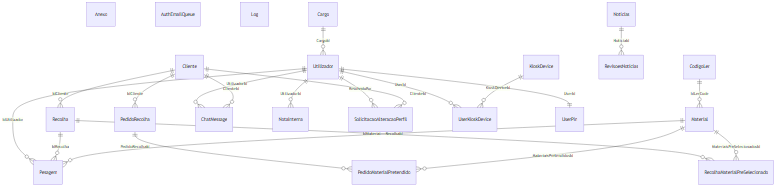
\includegraphics[width=0.9\textwidth]{imagens/erd.png}
    \caption{Diagrama de Entidade-Associação da base de dados centralizada.}
    \label{fig:erd}
\end{figure}

\subsection{Website Institucional}

O website institucional foi desenvolvido utilizando a versão 15 do Next.js com a arquitetura App Router. Esta escolha tecnológica permitiu tirar partido de renderização do lado do servidor (\textit{Server-Side Rendering}) e geração estática de páginas para otimizar o tempo de resposta inicial, garantindo simultaneamente boas práticas de indexação em motores de busca (SEO). A estilização e o desenho responsivo da interface foram concebidos com a versão 4 do Tailwind CSS, resultando numa interface moderna, fluida e adaptável a dispositivos móveis, tablets e computadores.

A plataforma está organizada em três grandes áreas funcionais e de acesso regulado: a área pública de informação e captação de clientes, a área reservada de clientes e o painel de administração de conteúdos.

\subsubsection{Área Pública}
A secção pública do website destina-se a apresentar os serviços da empresa e a estabelecer canais de comunicação com a comunidade e potenciais parceiros de negócio, sendo composta pelas seguintes páginas:
\begin{itemize}
    \item \textbf{Página Inicial:} Apresenta uma secção introdutória de forte impacto visual, um resumo dos serviços principais de recolha de resíduos industriais, estatísticas gerais sobre o impacto ecológico das atividades da empresa e uma secção de perguntas frequentes (FAQs) para responder rapidamente a dúvidas recorrentes dos utilizadores.
    \item \textbf{Serviços e Institucional:} Páginas dedicadas a detalhar os procedimentos regulamentares da empresa, os tipos de resíduos recolhidos e a história da organização.
    \item \textbf{Notícias:} Apresenta uma listagem cronológica de artigos publicados pela empresa, dotada de paginação e filtros de pesquisa por categorias, com redirecionamento para artigos de leitura individual.
    \item \textbf{Contactos:} Disponibiliza um canal direto de envio de mensagens com validação de dados e a integração de um mapa interativo para localização física das instalações da empresa.
    \item \textbf{Política de Privacidade:} Documento regulamentar para assegurar a conformidade da recolha e tratamento de dados dos utilizadores face à legislação em vigor.
\end{itemize}

\subsubsection{Área Reservada de Cliente}
Acedida através de mecanismos de autenticação segura, a área de cliente faculta aos parceiros comerciais ferramentas para gerir autonomamente as suas operações diárias com a empresa, dividindo-se nos seguintes módulos funcionais:
\begin{itemize}
    \item \textbf{Painel de Controlo:} Mostra um resumo dinâmico das recolhas efetuadas, pedidos ativos e alertas de suporte pendentes.
    \item \textbf{Pedidos de Recolha:} Permite a submissão de novas solicitações de recolha mediante um formulário onde o cliente indica os materiais de resíduos que deseja recolher, dados de contacto adicionais e anexa documentos ou fotografias relevantes para a operação. Disponibiliza ainda a consulta, cancelamento e reativação de pedidos em curso.
    \item \textbf{Histórico de Recolhas:} Regista os eventos logísticos concluídos e agendados. Apresenta o peso líquido total registado na balança física e a respetiva codificação legal (Lista Europeia de Resíduos), permitindo a exportação de dados em formatos estruturados como PDF e tabelas CSV.
    \item \textbf{Catálogo de Materiais:} Listagem paginada e pesquisável de todos os resíduos autorizados e geridos pela empresa, permitindo a exportação rápida dos dados tarifários vigentes para formato CSV.
    \item \textbf{Perfil de Cliente:} Permite ao parceiro solicitar atualizações aos seus dados cadastrais e fiscais. Estas alterações são submetidas a um fluxo de controlo interno, exigindo a aprovação manual de um operador no backoffice antes de serem efetivamente integradas na base de dados, prevenindo dados incorretos e tentativas de fraude.
    \item \textbf{Suporte Técnico (Chat):} Canal de mensagens direto e em tempo real com a equipa da empresa, concebido para acelerar a resolução de litígios ou o esclarecimento de dúvidas sobre agendamentos de recolha.
\end{itemize}

\subsubsection{Painel de Administração}
O painel administrativo é uma secção restrita e protegida por perfis de acesso elevados (administrador e super-administrador do website), que permite a gestão direta dos conteúdos editoriais do website:
\begin{itemize}
    \item \textbf{Módulo de Notícias:} Permite a criação, edição e eliminação lógica de publicações utilizando um editor visual de texto estruturado. Inclui campos dedicados para a configuração de títulos, slugs de URL e meta-descrições para a otimização em motores de busca (SEO).
    \item \textbf{Controlo e RevisoeseNoticias:} Possibilita a visualização do histórico de revisões dos artigos, permitindo comparar alterações estruturais e reverter edições antes da sua publicação definitiva no website.
\end{itemize}

\subsubsection{Alojamento e Publicação}
Durante as fases de desenvolvimento e testes de validação com a equipa da empresa, o website institucional foi alojado na plataforma Vercel, beneficiando de processos automatizados de compilação e publicação contínua (\textit{Continuous Deployment}). A arquitetura foi concebida para permitir a transição simplificada para o domínio e servidores corporativos permanentes da empresa.

\subsection{Ferramenta de Comparação de Preços de Toners}

No âmbito das necessidades de otimização do processo de vendas de consumíveis da empresa, foi desenvolvida uma ferramenta utilitária dedicada à comparação de preços de toners. Esta ferramenta permite carregar tabelas tarifárias e propostas de compra de múltiplos potenciais clientes corporativos e parceiros, frequentemente fornecidas em formatos de folhas de cálculo com diferentes estruturas de colunas, e efetuar o mapeamento flexível e a normalização de referências de produto. Com isto, a 20 Recolher consegue cruzar a informação do seu inventário de toners com a procura do mercado e com as tabelas de preços da concorrência, identificando a proposta de venda comercialmente mais vantajosa e competitiva para os seus compradores.

A aplicação foi construída utilizando a biblioteca React e a ferramenta de compilação Vite para a interface web. O processamento dos ficheiros locais é assegurado pela biblioteca XLSX, enquanto o armazenamento do histórico de tendências de preços é gerido localmente no navegador através de IndexedDB. Adicionalmente, foi implementada uma camada de empacotamento nativo com o Tauri para possibilitar a sua distribuição e execução como aplicação de ambiente de trabalho (\textit{desktop}). O desenvolvimento desta ferramenta foi realizado em parceria com o colega de estágio, tendo os testes unitários do motor de normalização de dados sido implementados com a biblioteca Vitest.

\subsection{App de Backoffice}

Para além do portal de clientes, o ecossistema tecnológico integra a aplicação de gestão interna (Backoffice), desenvolvida em .NET 10 sob a tecnologia Blazor Server. Esta aplicação destina-se ao controlo administrativo global da atividade e é utilizada pelos operadores e administradores da empresa para gerir e monitorizar todo o fluxo logístico e de pesagens.

A aplicação encontra-se estruturada nos seguintes módulos funcionais principais:
\begin{itemize}
    \item \textbf{Gestão de Entidades:} Permite o controlo de registos cadastrais de clientes e utilizadores do sistema, bem como a definição e atribuição de cargos e permissões de acesso estruturadas de forma granular para garantir a segurança lógica do sistema.
    \item \textbf{Controlo Logístico:} Módulo dedicado à triagem e agendamento de pedidos de recolha de resíduos, planeamento de recolhas e visualização dos dados consolidados de pesagens e quantidades processadas.
    \item \textbf{Auditoria de Segurança:} Regista e expõe os diários de atividade (\textit{audit logs}), detalhando todas as operações estruturais realizadas na base de dados (como criação, modificação ou inativação lógica de registos), identificando o utilizador responsável e o método de autenticação utilizado.
    \item \textbf{Validação de Alterações Cadastrais:} Canal onde os operadores analisam e validam ou rejeitam as solicitações de alteração de dados de identificação e faturação submetidas pelos clientes através da área reservada do website.
\end{itemize}

Em termos de usabilidade, a interface foi desenhada para se adaptar a diferentes cenários de trabalho, incluindo a utilização em dispositivos móveis e tablets no terreno. Para tal, implementaram-se tabelas de dados dinâmicas com colunas configuráveis e persistidas localmente para cada operador, além de menus de ações acionados por toque longo (\textit{long press}), adequados a ecrãs táteis. A aplicação disponibiliza ainda a exportação de relatórios de atividade em formato PDF e um painel dedicado à recuperação de registos inativos através do mecanismo de exclusão lógica (\textit{Soft-Delete}). O desenvolvimento desta aplicação de gestão foi realizado em colaboração com o colega de estágio.

\subsection{App de Balança - Terminal Kiosk}

Para além do backoffice administrativo, o sistema dispõe de um módulo dedicado especificamente à zona física de pesagens, designado por Terminal Kiosk. Trata-se de uma aplicação desenvolvida em .NET 10 sob a tecnologia Blazor Server, com uma interface otimizada para interação tátil (\textit{touchscreen}), concebida para ser operada de forma rápida e intuitiva por funcionários no terreno.

As características estruturais e operacionais deste terminal incluem:
\begin{itemize}
    \item \textbf{Integração com Balança Física:} O sistema comunica em tempo real com a balança industrial da empresa através de portas de comunicação série (protocolos RS-232), efetuando a leitura e importação automática do peso físico sem necessidade de introdução manual por parte do operador, o que minimiza erros humanos e otimiza o fluxo de registo.
    \item \textbf{Autenticação Simplificada:} A autenticação no quiosque é baseada na introdução de um código numérico pessoal (PIN) através de um teclado virtual sobredimensionado no ecrã. Isto evita a necessidade de introduzir palavras-passe complexas em ecrãs táteis expostos a poeira e condições operacionais de armazém.
    \item \textbf{Processo Guiado de Pesagem (Wizard):} O registo de pesagens é estruturado na forma de um assistente passo-a-passo (\textit{Wizard}). O operador seleciona a recolha em curso, o material que está a ser pesado, confirma a leitura automática do peso e submete o registo de forma sequencial e validada estruturalmente pelas regras de negócio.
    \item \textbf{Emparelhamento de Terminais (Pairing Code):} Para garantir que apenas quiosques físicos autorizados comunicam com a base de dados central, implementou-se um fluxo de emparelhamento obrigatório. O administrador gera um código de autorização temporário no backoffice e introduz este código no novo terminal para estabelecer a ligação encriptada definitiva.
\end{itemize}

A aplicação partilha componentes reutilizáveis através do módulo comum do projeto e foi desenhada com foco na usabilidade e fiabilidade das operações sob condições de armazém. O desenvolvimento deste módulo foi realizado em estreita parceria com o colega de estágio.

\subsection{Integração entre Sistemas e API Central}

Inicialmente, as aplicações de backoffice administrativo e o terminal de pesagem física (Kiosk) foram concebidos e implementados de forma acoplada numa única aplicação. No entanto, a evolução do projeto e a necessidade de isolar os ambientes físico e de escritório exigiram a separação destas ferramentas em duas aplicações independentes. Para suportar esta nova topologia sem comprometer a consistência dos dados, foi desenvolvida a API Central (\texttt{RecolherApp.Api}) na plataforma .NET.

Esta API funciona como a única interface de comunicação com a base de dados relacional e expõe um conjunto de serviços RESTful consumidos por todos os componentes do ecossistema, incluindo o website institucional. A arquitetura global do sistema segue os princípios da \textit{Clean Architecture}, dividindo-se em seis camadas estruturais:
\begin{itemize}
    \item \textbf{\texttt{RecolherApp.Api}:} Camada de exposição que gere os pontos de entrada (\textit{endpoints}), tratamento de pedidos HTTP e serialização de dados.
    \item \textbf{\texttt{RecolherApp.Core}:} Núcleo do domínio que contém a definição das entidades de negócio, validações estruturais e interfaces de repositórios.
    \item \textbf{\texttt{RecolherApp.Infrastructure}:} Implementação de acessos estruturais a bases de dados (via EF Core) e integrações com o serviço de armazenamento de objetos (Supabase Storage).
    \item \textbf{\texttt{RecolherApp.UI}:} Interface de utilizador do painel de backoffice (Blazor Server).
    \item \textbf{\texttt{RecolherApp.UI.Pesagens}:} Interface de utilizador do quiosque de balança (Blazor Server).
    \item \textbf{\texttt{RecolherApp.UI.Shared}:} Biblioteca partilhada contendo componentes de interface reutilizáveis (como assistentes, menus e inputs táteis) e tipos de dados comuns às duas aplicações Blazor.
\end{itemize}

O website institucional em Next.js também comunica de forma estrita com esta API central, sem nunca aceder diretamente à base de dados PostgreSQL. O fluxo de integração de pedidos de recolha funciona da seguinte forma:
\begin{enumerate}
    \item O cliente preenche e submete o formulário de recolha na área reservada do website.
    \item O servidor Next.js recebe o pedido e utiliza uma camada de proxy interna (\texttt{src/proxy.js}) para reencaminhar a solicitação para a API .NET, anexando de forma segura o token JWT de autenticação do cliente.
    \item A API central valida os dados estruturais do pedido, atualiza a base de dados relacional e aciona a fila de processamento assíncrono para o envio automático de e-mails cadastrais.
    \item O novo pedido passa imediatamente a estar visível no painel administrativo de backoffice para fins de agendamento logístico.
\end{enumerate}

Adicionalmente, a API disponibiliza o catálogo de materiais regulamentares para popular as seleções de formulários no website, integrando um mecanismo de salvaguarda local (\textit{local fallback}) para manter o formulário de pedidos funcional em caso de instabilidade temporária na ligação de rede. O envio de ficheiros e comprovativos no website é reencaminhado pelo proxy para a API .NET, que executa tarefas automáticas de compressão e conversão de imagem para o formato WebP antes de submeter os ficheiros para o armazenamento permanente no Supabase Storage.

\subsection{Segurança e Autenticação}

Para proteger os dados cadastrais, comerciais e operacionais geridos pelas diferentes aplicações, foi implementado um modelo de segurança e autenticação estruturado em duas vertentes principais: uma destinada ao portal web público e de clientes, e outra direcionada às ferramentas internas da empresa (Backoffice e quiosque de pesagens).

\subsubsection{Segurança no Website e Área de Cliente}
A autenticação e autorização na área de cliente e no painel administrativo do website são geridas através da integração com o serviço centralizado Supabase Auth, estruturando-se da seguinte forma:
\begin{itemize}
    \item \textbf{Criação de Conta via Convite:} O processo de registo de um novo cliente é acionado automaticamente aquando da submissão do seu primeiro pedido de recolha de resíduos. O sistema regista os dados na base de dados e insere uma tarefa na fila de envio de e-mails, disparando um convite seguro contendo um link de ativação único. O utilizador utiliza esse link para definir a sua palavra-passe e ativar a sua área reservada.
    \item \textbf{Gestão de Sessões com Tokens JWT:} Após a autenticação com sucesso, o sistema emite tokens JSON Web Token (JWT) que atestam a identidade e perfil do utilizador. Estes tokens são transmitidos e armazenados de forma segura utilizando cookies configurados com a propriedade \textit{HttpOnly}, garantindo que o código JavaScript do lado do cliente não tem acesso aos dados de sessão e prevenindo vulnerabilidades de roubo de credenciais.
    \item \textbf{Proteção de Rotas via Middleware:} O acesso às páginas privadas (tanto da área reservada de cliente como da administração) é interceptado por um componente de filtragem do Next.js (Middleware). Este componente valida a integridade do token, o seu prazo de validade e o perfil associado ao utilizador antes de permitir a renderização das páginas.
\end{itemize}

\subsubsection{Segurança nas Aplicações .NET (Backoffice e Quiosque)}
As ferramentas administrativas internas e de pesagem utilizam um modelo de autenticação adaptado às condições do ambiente onde são utilizadas:
\begin{itemize}
    \item \textbf{Autenticação por Código de Acesso (PIN):} No terminal quiosque de pesagem física, os operadores autenticam-se através de um código numérico pessoal. O sistema armazena este código encriptado recorrendo a algoritmos de dispersão (\textit{hashing}) seguros, impedindo a sua extração direta em caso de acesso indevido à base de dados estrutural.
    \item \textbf{Autorização de Quiosques (Pairing Code):} Para prevenir acessos não autorizados a partir de dispositivos físicos desconhecidos, a comunicação de novos quiosques com a API exige um processo de emparelhamento estruturado. O administrador gera um código temporário no backoffice e introduz este código no novo terminal para associar permanentemente o identificador do quiosque à lista de dispositivos autorizados.
    \item \textbf{Controlo de Acesso Baseado em Perfis:} A autorização interna baseia-se num sistema de controlo de acessos baseado em permissões granulares. Cada cargo profissional possui um conjunto de permissões ativas estruturado em formato JSON. Após a autenticação, a API central emite um token de sessão interno que transporta estas permissões e que é validado em cada pedido efetuado pelas aplicações Blazor.
\end{itemize}

\subsection{Resultados do Website Institucional}

Nesta secção, apresentam-se os resultados visuais e operacionais obtidos com a implementação do website institucional da empresa, ilustrando o estado final das principais interfaces e fluxos disponíveis.

A página principal do website (Figura~\ref{fig:homepage}) constitui a face pública da empresa. O seu desenho foca-se na facilidade de navegação e na promoção visual da marca, estruturando-se com um cabeçalho fixo com efeito de transparência, secções informativas de serviços e estatísticas gerais sobre o impacto ecológico das atividades de gestão de resíduos da empresa.

\begin{figure}[H]
    \centering
    \framebox[0.9\textwidth]{\parbox{0.85\textwidth}{\centering\vspace{1cm}[Captura de Ecrã: Homepage]\vspace{1cm}}}
    \caption{Interface pública da Página Inicial (Homepage) do website institucional.}
    \label{fig:homepage}
\end{figure}

A interface da área reservada de cliente (Figura~\ref{fig:dashboard}) oferece aos utilizadores autenticados um painel consolidado com a síntese de toda a sua atividade recente. Este ecrã organiza cartões informativos com métricas agregadas e atalhos rápidos para as secções operacionais principais, facilitando a gestão do histórico e pedidos.

\begin{figure}[H]
    \centering
    \framebox[0.9\textwidth]{\parbox{0.85\textwidth}{\centering\vspace{1cm}[Captura de Ecrã: Área de Cliente - Dashboard]\vspace{1cm}}}
    \caption{Ecrã do Painel de Controlo (Dashboard) na área reservada de cliente.}
    \label{fig:dashboard}
\end{figure}

O formulário de submissão de pedidos de recolha (Figura~\ref{fig:novopedido}) permite ao cliente registar uma nova solicitação de forma guiadca. O ecrã dispõe de controlos de seleção de locais de recolha, escolha paginada de materiais regulamentares e uma área dedicada ao carregamento de ficheiros para anexar imagens ou comprovativos de suporte.

\begin{figure}[H]
    \centering
    \framebox[0.9\textwidth]{\parbox{0.85\textwidth}{\centering\vspace{1cm}[Captura de Ecrã: Novo Pedido de Recolha]\vspace{1cm}}}
    \caption{Formulário de submissão de um novo pedido de recolha de resíduos.}
    \label{fig:novopedido}
\end{figure}

Por fim, o painel de administração de notícias (Figura~\ref{fig:adminnews}) é acessível a utilizadores administrativos e disponibiliza uma interface para gerir os conteúdos editoriais do site. O ecrã exibe a tabela de publicações, estatísticas básicas de leitura e botões de ação para abrir o editor de texto estruturado ou o histórico de revisões de artigos.

\begin{figure}[H]
    \centering
    \framebox[0.9\textwidth]{\parbox{0.85\textwidth}{\centering\vspace{1cm}[Captura de Ecrã: Painel Admin - Notícias]\vspace{1cm}}}
    \caption{Painel administrativo de gestão de publicações e notícias do website.}
    \label{fig:adminnews}
\end{figure}

\subsection{Resultados das Apps .NET}

Abaixo são descritos os ecrãs e resultados operacionais desenvolvidos para as aplicações em .NET 10 (Backoffice administrativo e quiosque tátil de balança), que suportam a gestão operacional interna.

O dashboard central da aplicação de Backoffice (Figura~\ref{fig:backoffice}) concentra as listagens de clientes e agendamentos logísticos. A interface exibe tabelas com dados dinâmicos e ordenáveis, contendo menus de ação contextual ativados por toque longo, que facilitam a edição e o processamento de recolhas e a visualização do histórico de auditoria.

\begin{figure}[H]
    \centering
    \framebox[0.9\textwidth]{\parbox{0.85\textwidth}{\centering\vspace{1cm}[Captura de Ecrã: Backoffice - Gestão de Recolhas]\vspace{1cm}}}
    \caption{Interface principal de gestão de recolhas no painel de Backoffice.}
    \label{fig:backoffice}
\end{figure}

O ecrã de entrada do quiosque tátil de balança (Figura~\ref{fig:kiosklogin}) é otimizado para ecrãs táteis em ambiente industrial. Apresenta botões sobredimensionados e um teclado numérico virtual que permite aos operadores introduzir o seu código de acesso pessoal PIN sem necessidade de periféricos físicos, garantindo a proteção e o controlo de acessos.

\begin{figure}[H]
    \centering
    \framebox[0.9\textwidth]{\parbox{0.85\textwidth}{\centering\vspace{1cm}[Captura de Ecrã: Quiosque - Login]\vspace{1cm}}}
    \caption{Interface de login tátil por PIN do quiosque físico de balança.}
    \label{fig:kiosklogin}
\end{figure}

O assistente de registo de pesagens no quiosque (Figura~\ref{fig:kioskweigh}) orienta o funcionário ao longo das fases de pesagem física. O assistente exibe em tempo real o valor lido a partir da balança industrial ligada por porta série, permitindo a seleção do tipo de resíduo e a confirmação do registo estruturado da recolha.

\begin{figure}[H]
    \centering
    \framebox[0.9\textwidth]{\parbox{0.85\textwidth}{\centering\vspace{1cm}[Captura de Ecrã: Quiosque - Pesagem]\vspace{1cm}}}
    \caption{Assistente de pesagem com leitura de peso automática via porta série.}
    \label{fig:kioskweigh}
\end{figure}

\section{Manutenção e Triagem de Hardware}

Paralelamente às tarefas de desenvolvimento de software, foram realizadas diversas atividades práticas e manuais no departamento técnico da empresa, focadas no processamento, triagem e recondicionamento de REEE. Estas atividades visam a economia circular, procurando testar e recuperar componentes funcionais antes de os encaminhar para reciclagem de matérias-primas.

\subsection{Testes e Diagnóstico de Memórias RAM}

A triagem de módulos de memória RAM constitui um passo essencial na recuperação de computadores obsoletos ou danificados que são entregues na empresa. Foram efetuados testes sistemáticos a memórias de tecnologia DDR3 e DDR4, tanto de formato DIMM (computadores de secretária) como SO-DIMM (portáteis). O processo estruturou-se da seguinte forma:
\begin{itemize}
    \item \textbf{Inspeção Visual Inicial e Limpeza:} Verificação de danos físicos no circuito impresso, contactos oxidados ou ausência de componentes passivos (como condensadores SMD). Os contactos dourados foram limpos de forma a remover qualquer oxidação.
    \item \textbf{Verificação de Funcionamento Prático:} Instalação de cada módulo individual numa placa-mãe/computador de teste compatível e ligação do equipamento. Caso o sistema arrancasse com sucesso e apresentasse imagem no ecrã (sinal de vídeo/POST), o módulo era validado como funcional.
    \item \textbf{Classificação e Armazenamento:} Os módulos aprovados foram classificados de acordo com a sua capacidade (GB) e tecnologia (DDR3 ou DDR4) e organizados para reutilização em equipamentos recondicionados. Módulos que não geravam imagem foram descartados e encaminhados para reciclagem de REEE.
\end{itemize}

\subsection{Testes de Unidades de Armazenamento (SATA SSD e M.2)}

Com a crescente substituição de discos mecânicos por unidades de estado sólido, a empresa recebe volumes significativos de dispositivos de armazenamento SSD, tanto com interface SATA de 2,5 polegadas como no formato M.2 (SATA e NVMe). Para avaliar a sua viabilidade de reutilização, seguiu-se o seguinte protocolo:
\begin{itemize}
    \item \textbf{Ligação e Apagamento de Dados:} Ligação das unidades a computadores de teste ou adaptadores dedicados. Efetuou-se uma formatação de baixo nível ou apagamento seguro para garantir a eliminação de dados anteriores e preservar a confidencialidade das informações de antigos utilizadores.
    \item \textbf{Análise de Saúde S.M.A.R.T.:} Execução do software Hard Disk Sentinel para ler os dados de integridade recorrendo à tecnologia SMART do disco. Foram avaliados a percentagem de saúde do dispositivo, o número de setores danificados e o tempo de atividade acumulado.
    \item \textbf{Destino das Unidades:} Unidades em excelente estado de saúde (normalmente com saúde superior a 80%) foram catalogadas e separadas para recondicionamento. Discos inoperacionais ou com níveis severos de degradação foram separados para reciclagem.
\end{itemize}

\subsection{Triagem e Separação de Baterias de Portáteis}

As baterias de iões de lítio (Li-ion) provenientes de computadores portáteis exigem um processo de triagem cuidadoso devido aos riscos de segurança associados ao seu armazenamento e transporte (risco de curto-circuito ou fuga térmica). As atividades realizadas nesta área englobaram:
\begin{itemize}
    \item \textbf{Triagem por Estado Físico:} Inspeção visual minuciosa para deteção de baterias com fissuras, fugas de eletrólito ou sinais de inchaço (deformação física). As baterias danificadas ou inchadas foram imediatamente isoladas e depositadas num bidão fechado e seguro, próprio para resíduos perigosos e inflamáveis.
    \item \textbf{Isolamento dos Terminais:} Aplicação sistemática de fita isoladora sobre os pinos de contacto de cada bateria para evitar o contacto acidental entre os terminais e mitigar riscos de curto-circuito durante o manuseamento e armazenamento.
    \item \textbf{Separação por Marca:} Organização das baterias em bom estado físico de acordo com o fabricante/marca do portátil correspondente (ex: HP, Dell, Asus, Lenovo), facilitando o seu emparelhamento com futuros equipamentos a recondicionar.
\end{itemize}

\subsection{Separação e Validação de Transformadores de Alimentação}

A triagem de transformadores (carregadores de computadores portáteis e periféricos diversos) permitiu recuperar centenas de unidades funcionais, evitando o desperdício de componentes elétricos de alta qualidade. O trabalho manual desenvolvido incluiu:
\begin{itemize}
    \item \textbf{Inspeção de Segurança Elétrica:} Exclusão de transformadores que apresentassem danos físicos visíveis na carcaça plástica ou cabos descarnados, dobrados ou cortados.
    \item \textbf{Teste Dinâmico de Alimentação:} Para verificar a integridade da entrega de energia, utilizou-se um computador de testes que se encontrava sem componentes internos como memórias RAM ou processador. Ao ligar o transformador à entrada de alimentação do computador de testes, a receção de energia fazia com que a placa-mãe emitisse um sinal sonoro (apito). A emissão deste som confirmava que o transformador estava a fornecer energia em conformidade.
    \item \textbf{Separação por Marca e Tipo de Conetor:} Triagem e catalogação das unidades aprovadas segundo a marca e o formato geométrico do conector de entrada (ex: conectores cilíndricos de diferentes diâmetros, fichas retangulares proprietárias ou interfaces USB-C), preparando-as para acompanhar equipamentos recondicionados ou para a reciclagem de cobre no caso dos componentes danificados.
\end{itemize}
